%Settings {{{
\documentclass[final]{beamer}
\usepackage[orientation=portrait,size=a1,scale=1,debug]{beamerposter}
\usepackage[T1]{fontenc}
\usepackage{lmodern}
\usetheme{gemini}
\usecolortheme{ox}
\usepackage{graphicx}
\usepackage{booktabs}
\usepackage{tikz}
\usepackage{pgfplots}
\pgfplotsset{compat=1.14}
\usepackage{anyfontsize}

%\setsansfont{FoundSteBoo}
%default font setup for use with pdflatex
%\renewcommand{\rmdefault}{phv} %%% Helvetica (very similar to Arial)


% ====================
% Lengths
% ====================

% If you have N columns, choose \sepwidth and \colwidth such that
% (N+1)*\sepwidth + N*\colwidth = \paperwidth
\newlength{\sepwidth}
\newlength{\colwidth}
\setlength{\sepwidth}{0.025\paperwidth}
\setlength{\colwidth}{0.3\paperwidth}

\newcommand{\separatorcolumn}{\begin{column}{\sepwidth}\end{column}}

\footercontent{
  XXXReferences and fundersXXX \hfill
  SAMOP 2023, \hfill
  \href{mailto:donovan.webb@physics.ox.ac.uk}{donovan.webb@physics.ox.ac.uk}}

% ====================
% Logo (optional)
% ====================

% use this to include logos on the left and/or right side of the header:
% \logoright{
\includegraphics[height=7cm]{logo1.pdf}}
\logoleft{\fbox{
    
\includegraphics[height=7cm]{figs/oxlogo.pdf}}
}

\newcommand{\SubItem}[1]{
    {\setlength\itemindent{15pt} \item[] #1}
}

%}}}

%title {{{

\title[FastGates]{\Huge Next generation platform for implementing fast gates in ion trap quantum computation}
\author{\textbf{D. Webb \and O. Bazavan \and S. Saner \and C. Ballance}}
\institute[]{
Ion Trap Quantum Computing Group,
Department of Physics, University of Oxford}

\begin{document}
\begin{frame}{} 
%}}}

\begin{center}

%Abstract {{{

    \vspace{-1em}
    \begin{block}{}
    \large
    Scalable trapped-ion quantum computation relies on the development of
    high-fidelity fast entangling gates in a many ion
    crystal. Conventional geometric phase gates either suffer from
    scattering errors or off-resonant carrier excitations. A potential
    route to achieve fast entanglement is creating a standing wave which
    can suppress the unwanted carrier coupling. \\

    %% We present the roadmap to our next-generation platform tailored for
    %% fast gates in the ~1us regime where gate speeds become comparable to
    %% the secular trap frequency. The quadrupole transitions between S1/2
    %% and D5/2 levels in Calcium 40 will be driven to perform
    %% Molmer-Sorenson gates with a standing wave rather than a typical
    %% travelling wave. The off-resonant carrier excitation may be strongly
    %% suppressed by placing ions at the nodes of the optical lattice. This
    %% new platform has scope for a multi-ion chain and a corresponding array
    %% of optical lattices which each address a single ion. The lattice array
    %% is created by a set of counter-propagating beams which are tightly
    %% focused by a symmetric setup of high-NA lenses. Control of the optical
    %% phase at the ion site will be achieved by actively stabilising the
    %% counter-propagating beam interferometer and feedbacking on the ion
    %% signal.
    \end{block}
%}}}

\begin{columns}[t]
  \begin{column}{0.49\textwidth}

%Why {{{
    \begin{alertblock}{Why Fast Gates?}
      \begin{itemize}
      \item Two qubit gates are implemented by coupling spin with motion of ions in the trap
      potential.

      \item Mølmer Sørenson (MS) interactions achieve this via a
      bichromatic field incident on the ions. Using travelling
      waves gives the Hamiltonian
      \Large$$ \hat{H}_{MS-TW} = \hbar\Omega \hat{S}_{\phi-\pi/2}\cos{(\delta t)} + \hbar\Omega\eta \hat{S}_\phi\cos{(\delta t)}(\hat{a}e^{-i\omega_zt} + \hat{a}^\dagger e^{i\omega_zt})$$\normalsize
      \vspace{0.4em}
      with the first term being the carrier whilst the second is the desired coupling.\vspace{0.8em}

      \item Fast entangling gates in ion traps enable the
            performance of complex quantum computations in reasonable times.\vspace{0.8em}

      \item However going fast requires moving out of the adiabatic
            regime. With travelling wave MS gates this results in errors
            due to both the presence of the carrier term and exciting
            ``spectator'' modes.\vspace{0.4em}

      \item Moving into the ??interaction picture?? this Hamiltonian
            may be expressed as [Xref Canzz?X]:
      \Large$$ \hat{H}_{MS-TW} = \hbar\eta\Omega(J_0(2\Omega/\delta) + J_2(2\Omega/\delta))\cdot \cos{(\delta t)}\hat{S}_{\phi}(\hat{a}e^{-i\omega_zt} + \hat{a}^\dagger e^{i\omega_zt})$$\normalsize
      \end{itemize}
      \begin{minipage}{0.58\textwidth}
      \begin{itemize}
      \item \textbf{Carrier term:} Error results in the effective rabi
        frequency being modulated by $(J_0 + J_2)$. This may be
        mitigated by supressing the carrier.\vspace{0.8em}

      \item \textbf{Spectator excitation:} Amplitude shaped pulses
        [ref vera] have been shown to effectively remove this
        ``spectator'' error by ensuring all the modes respective phase
        loops are closed on completion of the gate.\\
      \end{itemize}
      \end{minipage}
      \begin{minipage}{0.38\textwidth}
      \begin{figure}
        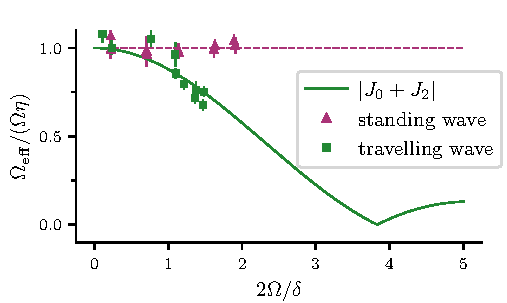
\includegraphics[width=0.98\textwidth]{./figs/J0J2.pdf}
      \end{figure}
      \end{minipage}

      \begin{figure}
        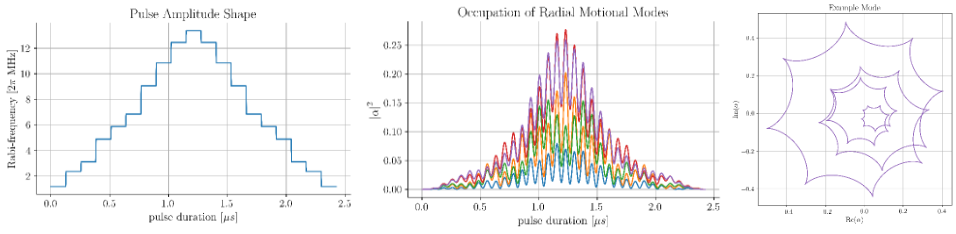
\includegraphics[width=0.9\textwidth]{./figs/loop_closing.png}
      \end{figure}
    \end{alertblock}
%}}}

%Lattice {{{
    \begin{alertblock}{Fast Gates with a Standing Wave}
      Bichromatic standing wave Hamiltonian where ions are seperated by $n\lambda$:

      \large$$ \hat{H}_{MS-SW} = \hbar 2\Omega \hat{S}_{\phi}\cos{(\delta t)}\sin{(\Delta\phi/2)} + \hbar 2\Omega\eta \hat{S}_\phi\cos{(\delta t)}(\hat{a}e^{-i\omega_zt} + \hat{a}^\dagger e^{i\omega_zt})\cos{(\Delta\phi/2)}$$\normalsize
      \begin{itemize}
      \item Setting $\Delta\phi = 0$ (ions sitting at antinodes) we
        entirely null the carrier term and maximise sideband
        coupling.\\
      \item Enables fast gates by preventing the saturation effect seen in the travelling MS.\\
      \item Using optical lattice gives complete control over phase visible to ions. \\
      \end{itemize}

      \begin{figure}
        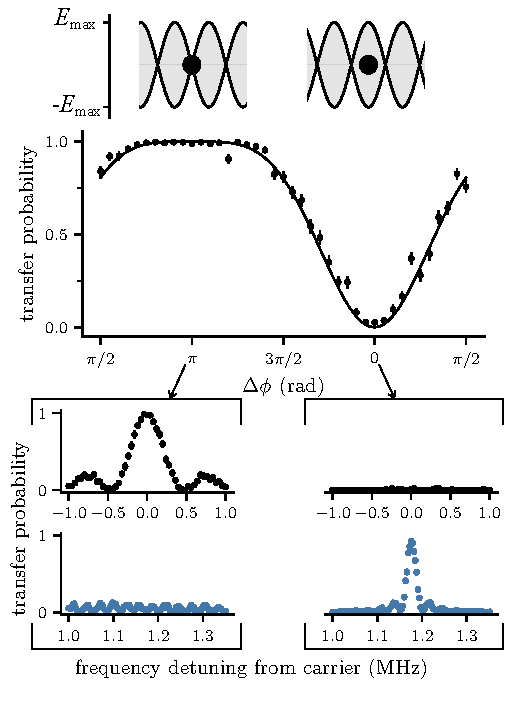
\includegraphics[width=0.48\textwidth]{./figs/Figure_2_v2.pdf}
        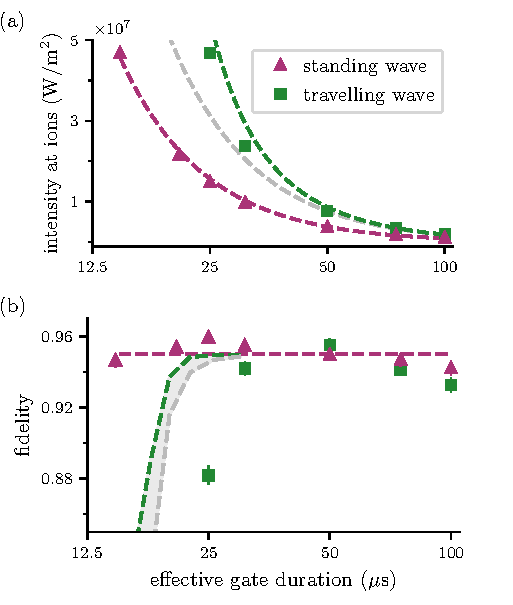
\includegraphics[width=0.48\textwidth]{./figs/two_qubit_gate_figure.pdf}
      \end{figure}

      Results from Cnulling:

    \end{alertblock}
%}}}

  \end{column}
  \begin{column}{0.49\textwidth}

%Experimental {{{
    \begin{alertblock}{$\mathbf{S_Z}$ type interactions}
      Talk about CANZZ
    \end{alertblock}

    \begin{alertblock}{Phase Stabilization}

      \begin{figure}
        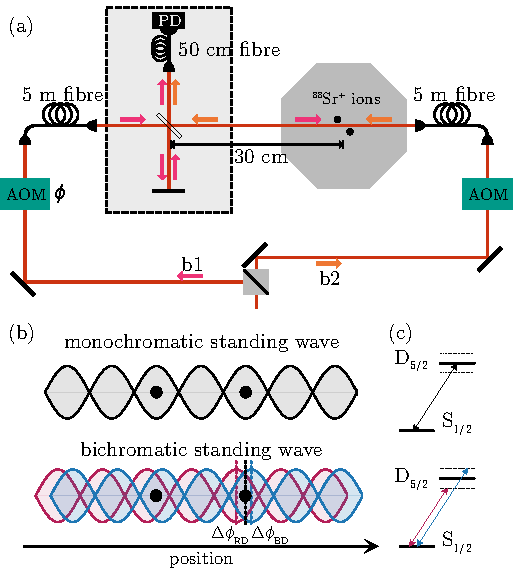
\includegraphics[width=0.5\textwidth]{./figs/setup+beams_horizontal.pdf}
      \end{figure}

      \begin{itemize}
      \item Optical lattice requires phase stabilisation to perform
            coherent interactions.\\
      \item Phase stabilised passively using enclosure and actively by two-step process:\\
      \SubItem 1) Fast drifts removed utilising interference of light
            from the two branches on a photodiode (PD).\\

      \SubItem 2) As PD lockpoint is ~30 cm away
            from ions, a second feedback loop using the ion as a
            sensor is required. We do this by performing a $\pi/2$-pulse
            using arm 1 ($\pi/2$, b1) followed immediately by a $\pi/2$-pulse
            using arm 2 ($pi/2$, b2). This is equivalent to a zero-delay
            Ramsey sequence, which gives a signal sensitive on the
            difference in phase between the two pulses, hence the
            relative phase be- tween the branches.\\

      \item No detriment using lattice: Standard Randomized
            Benchmarking gave quality of our single qubit rotations per
            gate to be $\epsilon = 0.173(3)\%$ for a travelling wave and
            $\epsilon = 0.144(3)\%$ for the standing wave.\\
      \end{itemize}
    \end{alertblock}


    \begin{alertblock}{New Platform}
      \begin{minipage}{0.58\textwidth}
      \begin{itemize}
      \item New ion trap experiment in development for exploring fast
        gate regime.
      \item Two high NA lenses allow optical
        access on both faces of the trap to create an array of singly
        addressing standing waves.
      \item 3D segmented trap design from NPL facilitates low heating
        rates whilst enabling ion shuttling and crystal rotations.
      \item Calcium 40
      \item quadropole transition used.
      \item MuMetal shield and permanent magnets.
      \item fig: solidworks of new experiment
      \end{itemize}
      \end{minipage}
      ~~
      \begin{minipage}{0.35\textwidth}
      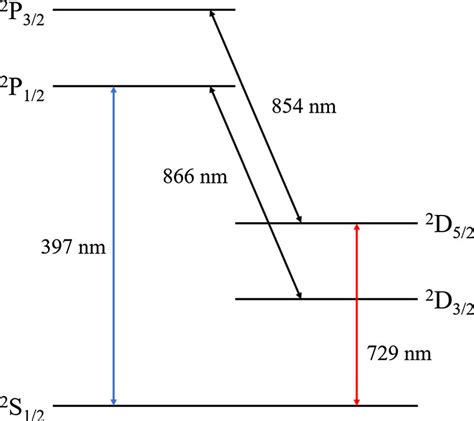
\includegraphics[width=0.94\textwidth]{./figs/ca_struct_tmp.jpeg}
      \end{minipage}

      \begin{figure}
        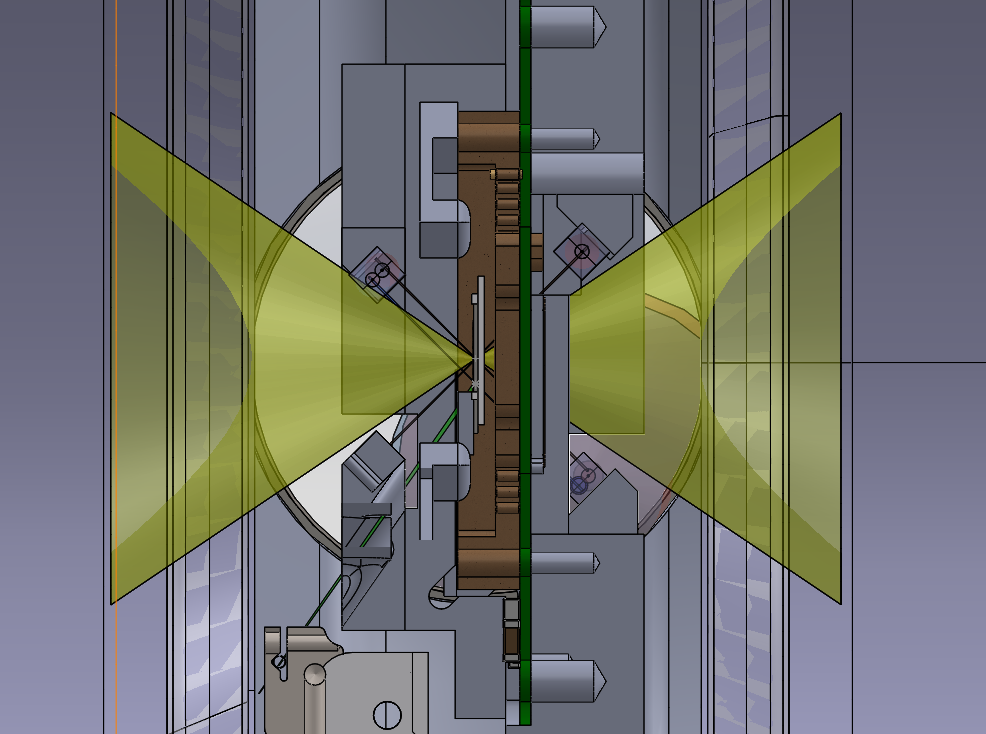
\includegraphics[height=0.35\textwidth]{./figs/trap_NA.png}
        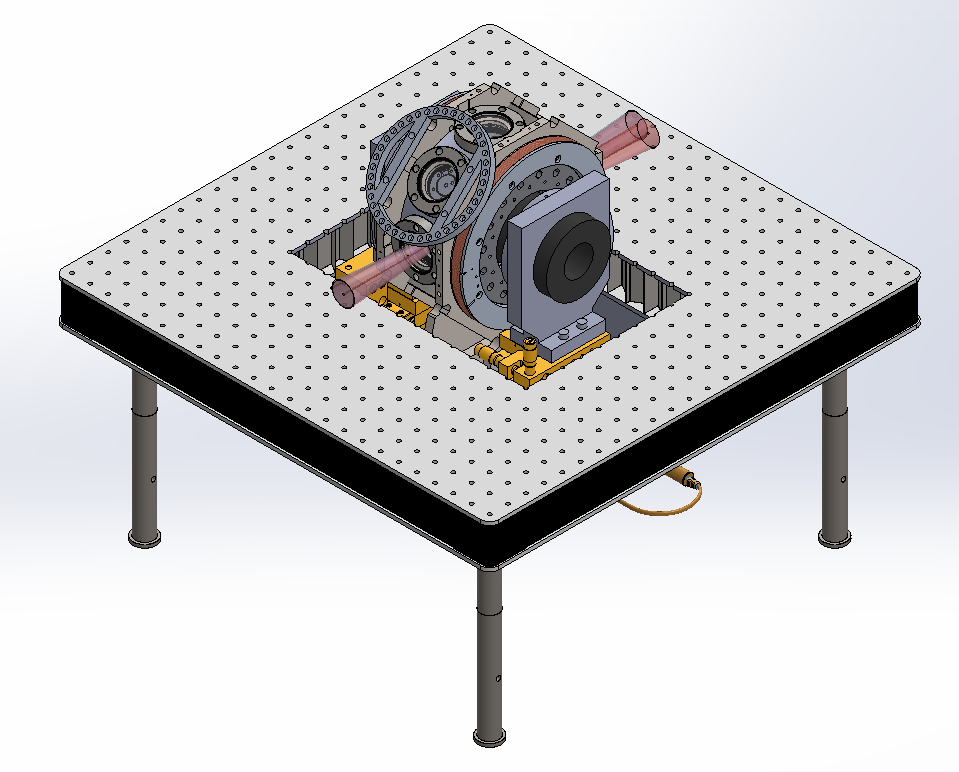
\includegraphics[height=0.35\textwidth]{./figs/exp_iso.png}
        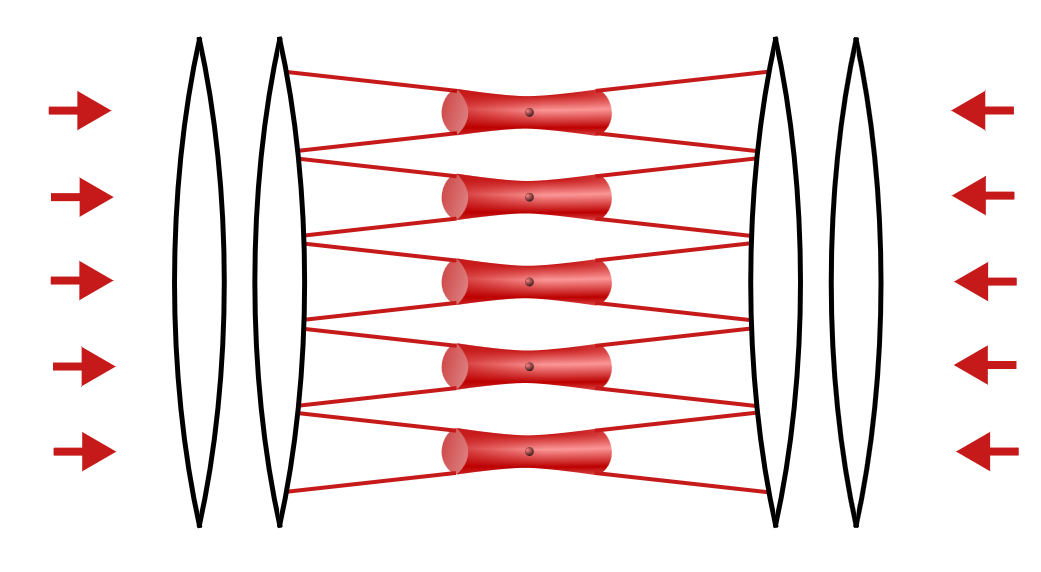
\includegraphics[height=0.35\textwidth]{./figs/array_sw.png}
      \end{figure}

    \end{alertblock}
%}}}

  \end{column}
\end{columns}
\end{center}

\end{frame}
\end{document}
